\section{Progress Conditions and Advice
Quantity}\label{progress-conditions-and-advice-quantity}

\begin{longtable}[]{@{}
  >{\raggedright\arraybackslash}p{(\linewidth - 6\tabcolsep) * \real{0.2500}}
  >{\raggedleft\arraybackslash}p{(\linewidth - 6\tabcolsep) * \real{0.2500}}
  >{\raggedleft\arraybackslash}p{(\linewidth - 6\tabcolsep) * \real{0.2500}}
  >{\raggedleft\arraybackslash}p{(\linewidth - 6\tabcolsep) * \real{0.2500}}@{}}
\caption{Separate ten-seed advice-quantity control. Thinned-full minus
no-progress AUC is +0.720 {[}0.526, 0.914{]}, Holm-adjusted
\(p=.000038\). The aggregate retained-label ratio is 1.0048. Per-run
label counts are rounded means. This cohort differs from the original
and fresh source cohorts.}\tabularnewline
\toprule\noalign{}
\begin{minipage}[b]{\linewidth}\raggedright
KeyCorridor-S3R3, plain PPO
\end{minipage} & \begin{minipage}[b]{\linewidth}\raggedleft
AUC
\end{minipage} & \begin{minipage}[b]{\linewidth}\raggedleft
Final success (\%)
\end{minipage} & \begin{minipage}[b]{\linewidth}\raggedleft
Retained labels per run
\end{minipage} \\
\midrule\noalign{}
\endfirsthead
\toprule\noalign{}
\begin{minipage}[b]{\linewidth}\raggedright
KeyCorridor-S3R3, plain PPO
\end{minipage} & \begin{minipage}[b]{\linewidth}\raggedleft
AUC
\end{minipage} & \begin{minipage}[b]{\linewidth}\raggedleft
Final success (\%)
\end{minipage} & \begin{minipage}[b]{\linewidth}\raggedleft
Retained labels per run
\end{minipage} \\
\midrule\noalign{}
\endhead
\bottomrule\noalign{}
\endlastfoot
No advice & .000 & 0.0 & 0 \\
Full bank & .722 & 90.0 & 1,465,562 \\
No progress conditions & .019 & 8.6 & 1,073,271 \\
Randomly thinned full bank & .739 & 89.6 & 1,078,445 \\
\end{longtable}

Random thinning approximately matches aggregate retained advice
quantity, while retaining a large learning advantage for
progress-conditioned advice. It does not match the states visited, the
individual targets or gradient estimates. The full-bank reference mean
is slightly below the thinned-bank mean; this descriptive difference
does not establish that thinning improves learning.


\begin{figure}[htbp]\centering
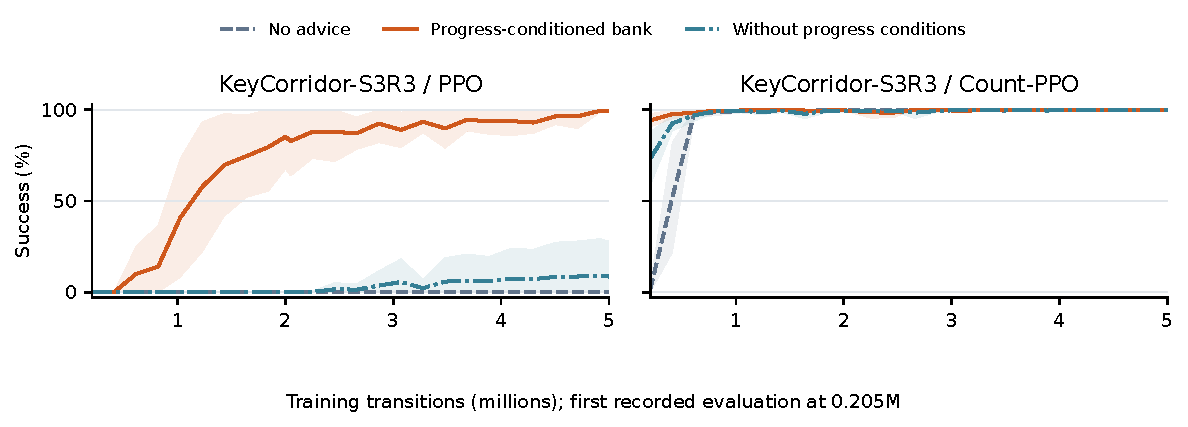
\includegraphics[width=\linewidth]{figures/progress_learning.pdf}
\caption{KeyCorridor progress-condition ablation, ten paired seeds and 5M transitions. Curves are mean teacher-free greedy success with pointwise unadjusted 95\% $t$-intervals across training seeds, clipped to the feasible range. Curve-band overlap is not a test of paired AUC differences.}
\end{figure}

\begin{figure}[htbp]\centering
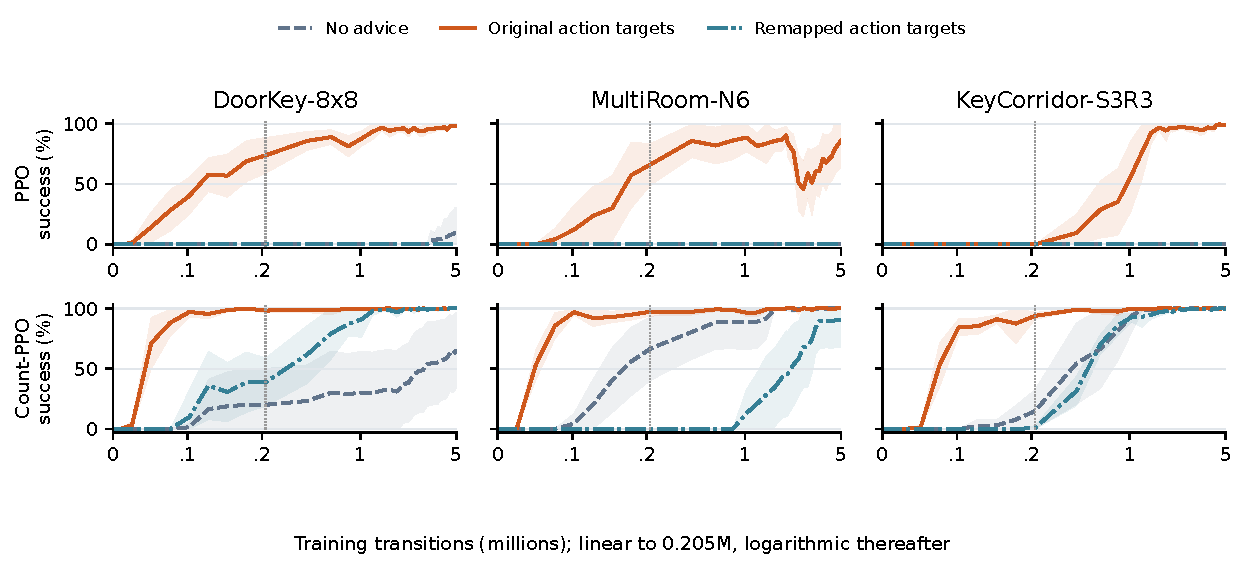
\includegraphics[width=\linewidth]{figures/content_learning.pdf}
\caption{Fresh action-content control, ten paired seeds per setting and 5M transitions. Measured initialization is included. The horizontal axis is linear through 204,800 transitions and logarithmic thereafter. Curves are mean teacher-free greedy success with pointwise unadjusted 95\% $t$-intervals across training seeds, clipped to the feasible range. Curve-band overlap is not a test of paired AUC differences.}
\end{figure}
